\toptitle{[ELEC-H-201] Électricité et électronique}{TP2}
\TPtitle{Électricité et électronique\vspace*{2mm}}{TP2:\vspace*{2mm}
Filtrage et amplification}

\frontpage{consignes2.tex}
\vspace{5cm}
\newpage

\section{Filtrage}
Dans cette première partie de la séance, nous verrons comment analyser un diagramme de Bode, comment comprendre et concevoir un filtre passif et comment en déduire les courbes de Bode.


\subsection{Analyse de diagrammes de Bode}
Un diagramme de Bode est une paire de courbes permettant de représenter la réponse en fréquence d'un système $H(j\omega)$, par exemple un filtre.
Cette réponse en fréquence est le rapport entre des grandeurs en entrée et en sortie du système, par exemple ses tensions~: $H(j\omega) = \frac{\underline{V}_{out}}{\underline{V}_{in}}$.
Étant donné que nous travaillons avec des grandeurs représentées par des phaseurs, nous allons séparer l'étude de l'amplitude et de la phase.

La première courbe est celle du \textbf{gain} et représente l'évolution de ce dernier en fonction de la fréquence $f$ ou de la pulsation $\omega$\footnote{Rappel~: $\omega = 2\pi \cdot f$} de la source à l'entrée du système.
Ce gain est le rapport des amplitudes des grandeurs étudiées et donc le module de la réponse en fréquence~: $|H(j\omega)| = \frac{|\underline{V}_{out}|}{|\underline{V}_{in}|}$.
Un gain supérieur à l'unité signifie que l'amplitude en sortie du système sera plus élevée qu'en entrée, on dira que le signal est \textit{amplifié}.
Un gain compris entre 0 et 1 signifie par contre que l'amplitude en sortie est plus faible qu'en entrée, on dira que le signal est \textit{atténué}.\\
On peut aussi exprimer ce gain naturel en \textit{décibel} en utilisant l'expression suivante~: $X [dB] = 20 \cdot log_{10}\left(\frac{|V_{out}|}{|V_{in}|}\right)$.
Dans ce cas, un gain supérieur à 0 dB sera dit amplifié et inférieur à 0 dB sera atténué.

La seconde courbe est celle de la \textbf{phase}, elle représente quant à elle l'évolution de la phase de la réponse en fréquence, c'est-à-dire son argument~: $Arg(H(j\omega)) = \frac{Arg(\underline{V}_{out})}{Arg(\underline{V}_{in})}$.
Si la phase est positive, on dira que la sortie est en \textit{avance} de phase sur l'entrée.
À l'inverse, si la phase est négative, on dira que la sortie est en \textit{retard} de phase.

\clearpage

\Question{0}
{
Sur les tracés suivants, quel est le gain naturel et en décibel pour 10~Hz, 1~kHz et 10~kHz ?

\begin{tikzpicture}[gnuplot def/.append style={prefix={}},xscale=7/4]% 7 cm horizontaly for 5 decades
 \tikzset{
 semilog lines/.style={black},
 semilog lines 2/.style={gray!50},
 semilog half lines/.style={gray!50, dotted},
 semilog label x/.style={below,font=\scriptsize},
 semilog label y/.style={above,font=\scriptsize},
 Bode lines/.style={very thick, blue} }
\begin{scope}[yscale=3/80] % 3 cm verticaly for 80 dB
\UnitedB
\def\Unitx{Hz}
\OrdBode{10}
\semilog{1}{5}{-40}{40}
\BodeGraph[]{1:5}{\POAmp{10}{0.01}}
\end{scope}
\begin{scope}[yshift=-4cm,yscale=3/80] % 3 cm verticaly for 80 dB
\UnitedB
\def\Unitx{Hz}
\OrdBode{10}
\semilog{1}{5}{-40}{40}
\BodeGraph[]{1:5}{-\POAmp{5}{0.001}}
\end{scope}
\begin{scope}[yshift=-8cm,yscale=3/80] % 3 cm verticaly for 80 dB
\UnitedB
\def\Unitx{Hz}
\OrdBode{10}
\semilog{1}{5}{-40}{40}
\BodeGraph[]{1:5}{-\IntAmp{10}+\POAmp{1}{0.01}}
\end{scope}
\end{tikzpicture}
}
{
  
  \begin{center}
  \begin{tabular}{cccc}
  Relevé & 10 Hz & 1 kHz & 10 kHz \\ \hline
  1 & 20 dB/10 & 0 dB/1 & -20 dB/0.1 \\
  2 & -12 dB/0.25 & -10 dB/0.32 & 8 dB/2.5 \\
  3 & 0 dB/1 & 20 dB/10 & 20 dB/10 \\
  \end{tabular}
  \end{center}
  Gain en dB/gain naturel
}

\clearpage

\Question{0}
{
Pour ces différents signaux d'entrée, quelle sera l'expression du signal de sortie étant donné le diagramme de Bode suivant pour le système ?
\begin{center}
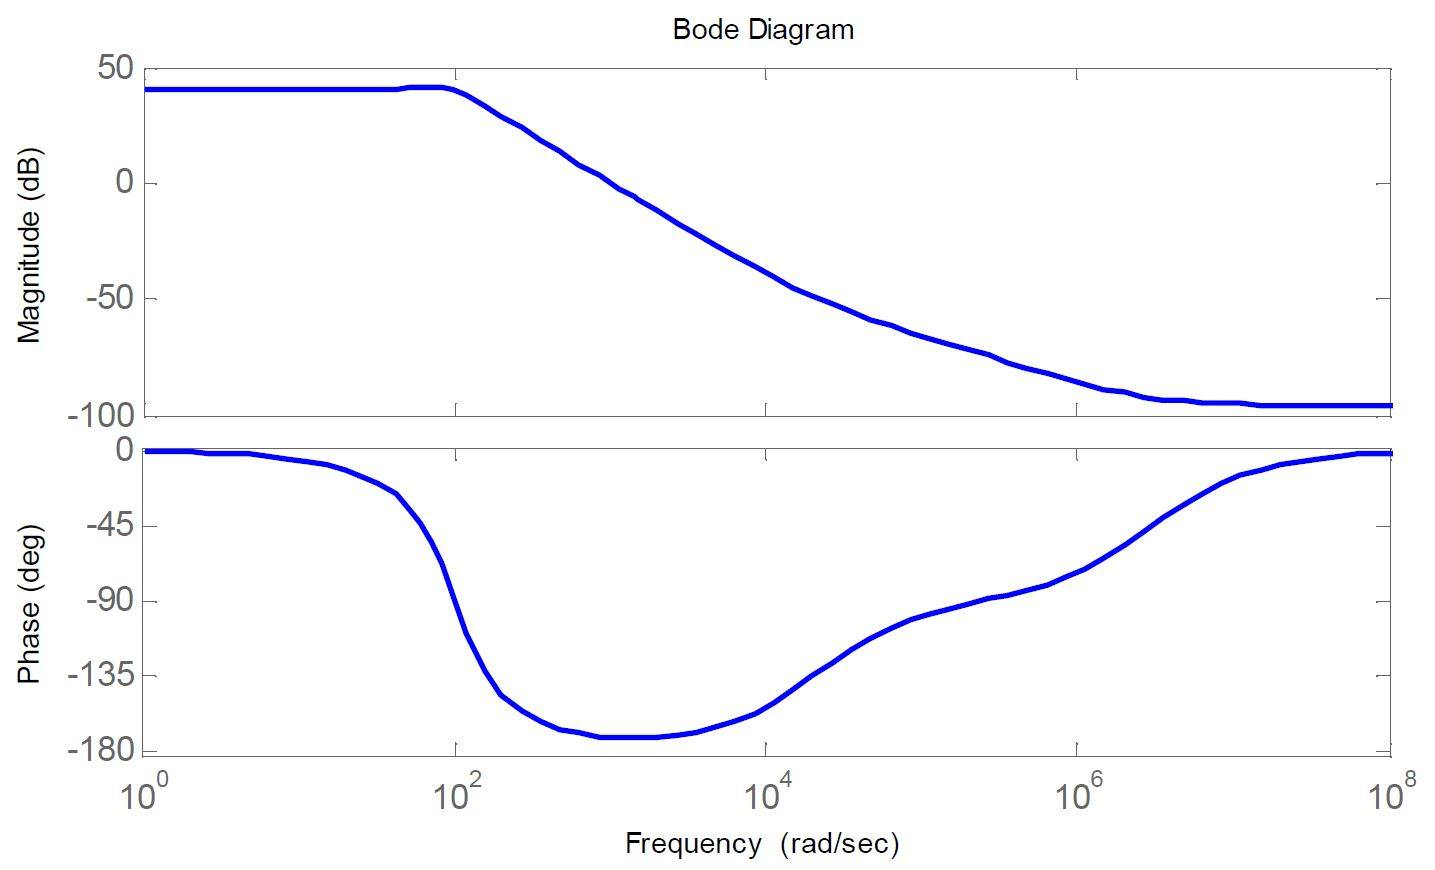
\includegraphics[width=12cm]{exo_bode}
\end{center}

\begin{enumerate}
\item $V_{in}(t)=1V\times cos(100\frac{rad}{s}t)$
\item $V_{in}(t)=5V\times cos(10^4\frac{rad}{s}t)$
\item $V_{in}(t)=2V\times cos(1000\frac{rad}{s}t+\frac{\pi}{6})$
\end{enumerate}
}
{
  \begin{enumerate}
    \item 45 dB et -90° : $V_{out}(t) = 177 V \times cos(100\frac{rad}{s}t - \frac{\pi}{2})$
    \item -50 dB et -145° : $V_{out}(t) = 16 mV\times cos(10^4\frac{rad}{s}t - \frac{145}{180}\pi)$
    \item 0 dB et -170° : $V_{out}(t) = 2 V\times cos(1000\frac{rad}{s}t - \frac{\pi}{6} - \frac{170}{180}\pi)$
  \end{enumerate}
}


\subsection{Filtre}
Un filtre électronique est un circuit  qui modifie le signal d'entrée en changeant sa phase ou son amplitude.
Plus particulièrement, nous allons aborder les filtres \textit{passifs}, c'est-à-dire fonctionnant sans alimentation autre que le signal d'entrée.
De tels filtres sont composés d'une combinaison de résistances, condensateurs et inductances.
Afin de déterminer le comportement du filtre, il convient d'établir sa \textbf{réponse en fréquence} $H(j\omega)$.

Prenons par exemple le circuit suivant composé de deux impédances générales $Z_1$ et $Z_2$~:

\begin{center}
  \begin{circuitikz} \draw
    (0,0) node[ground]{}
    to[american voltage source, v=$V_{in}$, invert] (0,3)
    to[generic, l=$Z_1$] (3,3)
    (3,0) to[generic, l=$Z_2$, v=$V_{out}$] (3,3)
    (3,0) -- (0,0);
  \end{circuitikz}
\end{center}

Nous retrouvons ici la configuration d'un diviseur impédant dont l'expression est la suivante~:
\[\underline{V}_{out} = \underline{V}_{in} \cdot \frac{Z_2}{Z_1 + Z_2}\]

Nous pouvons immédiatement en déduire l'expression de sa réponse en fréquence~:
\[H(j\omega) = \frac{\underline{V}_{out}}{\underline{V}_{in}} = \frac{Z_2}{Z_1 + Z_2}\]

\Question{0}
{
Quelle est l'expression de l'impédance du condensateur, de l'inductance et de la résistance ?
}
{
  $Z_R = R$, $Z_C = \frac{1}{j\omega C}$, $Z_L = j\omega L$
}

\Question{0}
{
Quelle est la réponse en fréquence des quatre filtres suivants~?
\begin{center}
  \begin{circuitikz}[scale=0.7] \draw
    (0,0) node[ground]{}
    to[american voltage source, v=$V_{in}$, invert] (0,3)
    to[C, l=$C$] (3,3)
    (3,0) to[R, l=$R$, v=$V_{out}$] (3,3)
    (3,0) -- (0,0);
  \end{circuitikz}\hspace*{1cm}
  \begin{circuitikz}[scale=0.7] \draw
    (0,0) node[ground]{}
    to[american voltage source, v=$V_{in}$, invert] (0,3)
    to[R, l=$R$] (3,3)
    (3,0) to[C, l=$C$, v=$V_{out}$] (3,3)
    (3,0) -- (0,0);
  \end{circuitikz}\hspace*{1cm}
\end{center}

\begin{center}
  \begin{circuitikz}[scale=0.7] \draw
    (0,0) node[ground]{}
    to[american voltage source, v=$V_{in}$, invert] (0,3)
    to[L, l=$L$] (3,3)
    (3,0) to[R, l=$R$, v=$V_{out}$] (3,3)
    (3,0) -- (0,0);
  \end{circuitikz}\hspace*{1cm}
  \begin{circuitikz}[scale=0.7] \draw
    (0,0) node[ground]{}
    to[american voltage source, v=$V_{in}$, invert] (0,3)
    to[R, l=$R$] (3,3)
    (3,0) to[L, l=$L$, v=$V_{out}$] (3,3)
    (3,0) -- (0,0);
  \end{circuitikz}\hspace*{1cm}
\end{center}
}
{
  \begin{itemize}
    \item RC avec sortie sur R : $H(j\omega) = \frac{j\omega R C}{1 + j\omega R C}$
    \item RC avec sortie sur C : $H(j\omega) = \frac{1}{1 + j\omega R C}$
    \item RL avec sortie sur R : $H(j\omega) = \frac{R}{R + j\omega L}$
    \item RL avec sortie sur L : $H(j\omega) = \frac{j\omega L}{R + j\omega L}$
  \end{itemize}
}

\subsubsection{Passe-haut ou passe-bas}

Chacun de ces filtres va laisser «~passer~» certaines fréquences (gain unitaire, soit 0 dB) et en atténuer d'autres (gain $\in [0,1[$, ou < 0 dB).
Ils ne présenteront jamais d'amplification (sauf en cas de résonance), étant donné qu'ils n'ont pas d'apport d'énergie.
Un filtre laissant passer les basses fréquences est dit \textbf{passe-bas}, tandis que s'il laisse passer les hautes fréquences, il sera \textbf{passe-haut}.
Pour déterminer le type d'un filtre, on peut procéder à une \textit{étude asymptotique}, c'est-à-dire étudier le module de la réponse en fréquence lorsque $\omega \rightarrow 0$ et $\omega \rightarrow \infty$.

\Question{0}
{
Quel est le type de chacun des filtres précédents ?
}
{
  \begin{center}
    \begin{tabular}{cccc}
    Filtre & $\omega \rightarrow 0$ & $\omega \rightarrow \infty$ & Type \\ \hline
    RC avec sortie sur R & $|H(j\omega)| = 0$ & $|H(j\omega)| = 1$ & Passe-haut \\
    RC avec sortie sur C & $|H(j\omega)| = 1$ & $|H(j\omega)| = 0$ & Passe-bas \\
    RL avec sortie sur R & $|H(j\omega)| = 1$ & $|H(j\omega)| = 0$ & Passe-bas \\
    RL avec sortie sur L & $|H(j\omega)| = 0$ & $|H(j\omega)| = 1$ & Passe-haut \\
    \end{tabular}
  \end{center}
}

\subsubsection{Fréquence de coupure}
De passant à bloquant, un filtre change de comportement à une fréquence particulière~: sa \textbf{fréquence de coupure} $f_c$ ou \textbf{pulsation de coupure} $\omega_c$.
Il y a trois manières différentes de déterminer cette fréquence particulière~:
\begin{enumerate}
  \item Par le temps caractéristique $\tau$ du circuit, sachant que $\omega_c = 1/\tau$.
  \item Par le gain à la fréquence de coupure, sachant que $|H(j\omega_c)| = 1/\sqrt{2} = -3 dB$.
  \item En connaissant les pôles et zéros de la réponse en fréquence.
\end{enumerate}
~\\

\Question{0}
{
Quel est le temps caractéristique\footnote{Il s'agit aussi de sa constante de charge.} d'un circuit RC~? D'un circuit RL~?
Déduisez-en les pulsations de coupure respectives.
}
{
  \begin{center}
    \begin{tabular}{ccc}
    Circuit & $\tau$ & $\omega_c$ \\ \hline
    RC & $RC$ & $1/RC$ \\
    RL & $L/R$ & $R/L$ \\
    \end{tabular}
  \end{center}
}

\Question{0}
{
Vérifiez que le gain à cette fréquence de coupure est de -3 dB pour les circuits RC et RL.
}
{
  \begin{itemize}
    \item RC avec sortie sur R : $H(j\omega) = \frac{j\omega R C}{1 + j\omega R C}$, donc $|H(j\omega)| = \frac{\omega R C}{\sqrt{1 + (\omega R C)^2}}$
    \item RC avec sortie sur C : $H(j\omega) = \frac{1}{1 + j\omega R C}$, donc $|H(j\omega)| = \frac{1}{\sqrt{1 + (\omega R C)^2}}$
    \item RL avec sortie sur R : $H(j\omega) = \frac{R}{R + j\omega L}$, donc $|H(j\omega)| = \frac{R}{\sqrt{R^2 + (\omega L)^2}}$
    \item RL avec sortie sur L : $H(j\omega) = \frac{j\omega L}{R + j\omega L}$, donc $|H(j\omega)| = \frac{\omega L}{\sqrt{R^2 + (\omega L)^2}}$
  \end{itemize}
}

Pour pouvoir utiliser la troisième méthode (pôles et zéros), il faut comprendre comment analyser une réponse en fréquence et en déduire le diagramme de Bode.

\subsection{Tracé du diagramme de Bode}

Pour obtenir le tracé, il faut passer par plusieurs étapes~:
\begin{enumerate}
  \item Mettre la réponse en fréquence sous sa forme canonique.
  \item Lister les pôles et zéros de la fonction, ainsi que leur degré respectif.
  \item Parcourir ces derniers dans leur ordre croissant pour construire les tracés \textit{asymptotiques}.
  \item Réaliser le tracé final sur base des asymptotes (généralement ignoré à main levée).
\end{enumerate}

\subsubsection{Forme canonique}
La forme canonique générale de réponse en fréquence est la suivante~:
\[H(j\omega) = \frac{ A_0\ (j\omega)^{k_0} \cdot \left(1 + \frac{j\omega}{z_1} \right)^{k_1} \dots \left(1 + \frac{j\omega}{z_n} \right)^{k_n} }{\left(1 + \frac{j\omega}{p_1} \right)^{k_{n+1}} \dots \left(1 + \frac{j\omega}{p_n} \right)^{k_{n+m}}}\]

Par exemple, si $H(j\omega) = \frac{j\omega L}{R + j\omega L}$, alors sa forme canonique sera 
\[H(j\omega) = \frac{j\omega L}{R + j\omega L} = \frac{L \cdot j\omega}{R\cdot \left(1 + \frac{j\omega L}{R}\right)} = \frac{L/R \cdot j\omega}{1 + \frac{j\omega}{R/L}}\]


\subsubsection{Identifier les pôles et zéros de la fonction}
Les \textbf{pôles} sont les termes permettant d'annuler le \textit{dénominateur} de la réponse en fréquence\footnote{Il s'agit d'un abus de langage utilisé dans ce cours, les pôles et zéros s'appliquent normalement à la fonction de \textit{transfert}.}, c'est-à-dire les termes $p_i$ dans la forme canonique\footnote{$1 + \frac{j\omega}{\sigma} = 0 \Leftrightarrow j\omega = -\sigma$, mais c'est bien sa \textbf{valeur absolue} qui nous intéresse. Il s'agit à nouveau d'une conséquence de l'abus d'équivalence entre fonction de transfert $H(p)$ et réponse en fréquence $H(j\omega)$.}.
Leur \textbf{degré} est l'exposant $k_i$ du groupe auquel ils appartiennent.
De la même manière, les \textbf{zéros} sont les termes $z_i$ de la forme canonique et annulent le numérateur.
Si $k_0 \neq 0$, on dira qu'on a un \textit{zéro à l'origine} si $k_0 > 0$ ou un \textit{pôle à l'origine} si $k_0 < 0$.

Dans notre exemple, nous avons un zéro à l'origine de degré 1 ($k_0 = 1$) et un pôle en $R/L$ de degré 1.

\subsubsection{Construction du tracé asymptotique}
Les pôles et zéros auront chacun une influence sur le tracé asymptotique, tant du gain que de la phase, en fonction de leur degré $k$.

\begin{center}\renewcommand{\arraystretch}{1.3}
\begin{tabular}{lcc}
& Gain & Phase \\ \hline
Zéro & Pente $+k$ & $+k\cdot90\degree$ \\
Pôle & Pente $-k$ & $-k\cdot90\degree$
\end{tabular}
\end{center}

Attention, il s'agit de \textbf{modifications successives} de la pente du gain et de la phase~!
Par exemple, si nous rencontrons un zéro de degré 1, il va \textit{modifier} la pente actuelle en lui ajoutant $+1$. Si cette dernière était de $-2$ à cause de pôles précédents, la nouvelle pente sera bien de $-2 + 1 = -1$. Le zéro n'aura \textbf{pas} fixé la valeur de la pente à $+1$.

Une pente de $+1$ signifie qu'une multiplication par 10 de la fréquence entraîne une multiplication par 10 du gain. Cette multiplication du gain correspond à une progression de $20\cdot log (10) = 20 dB$.
De plus, une multiplication (ou division) par 10 de la fréquence correspond à une \textbf{décade}. Par exemple, 100 Hz est une décade au-dessus de 10 Hz et deux décades en dessous de 10 kHz.
Dès lors, une pente de $+1$ correspond à $+20 dB/\mbox{décade}$.

Dans notre exemple, nous avons~:

\begin{itemize}
  \item Un zéro à l'origine de degré 1. La pente du gain commencera à $+1$ et la phase à $+90\degree$.
  \item Un pôle simple (degré 1) en $\omega = R/L$, la pente du gain devient $0$ et la phase $0\degree$.
\end{itemize}

\begin{center}
\begin{tikzpicture}[gnuplot def/.append style={prefix={}},xscale=7/4]% 7 cm horizontaly for 5 decades
 \tikzset{
 semilog lines/.style={black!70},
 semilog lines 2/.style={gray!50},
 semilog half lines/.style={gray!50, dotted},
 semilog label x/.style={below,font=\scriptsize},
 semilog label y/.style={above,font=\scriptsize},
 % every node/.style={font=\scriptsize},
 Bode lines/.style={very thick, blue},
 asymp lines/.style={Bode lines, very thick} }
\begin{scope}[yscale=3/80] % 3 cm verticaly for 80 dB
\UnitedB
% \def\Unitx{Hz}
\OrdBode{20}
\semilog{1}{5}{-60}{20}
\BodeGraph[]{1:5}{-\IntAmp{1000}+\POAmpAsymp{1}{0.001}} % High-pass
% \IntAmp{x} gives you the gain at w=10^0. So to have -60dB at 10^0, you need "-\IntAmp{1000}"
% \POAmpAsymp{1}{x} where x is w value of the pole/zero.

% \BodeGraph[]{1:5}{\POAmpAsymp{1}{0.01}} % Low-pass
% \BodeGraph[]{1:5}{\POAmp{10}{0.01}}
\node [ref points, label={[blue]above right:$\omega_c$}] at (3, -60) {};
\end{scope}
\begin{scope}[yshift=-5cm, yscale=3/270]
\UniteDegre
% \def\Unitx{Hz}
\OrdBode{90}
\semilog{1}{5}{-90}{180}
\BodeGraph[asymp lines,samples=100, const plot]{1:5}{-\IntArg{1000}+\POArgAsymp{1}{0.001}} % High-pass
% If the transition from one phase to another is not "straight" enough, you might not have enough samples or you forgot the "const plot" argument.
\node [ref points, label={[blue]above right:$\omega_c$}] at (3, -90) {};
\end{scope}
\end{tikzpicture}
\end{center}

Le gain du plateau (pente nulle) du tracé du gain peut-être obtenu en faisant tendre $\omega \rightarrow \infty$, ce qui nous donne 1 ou 0 dB.


Nous remarquons ainsi que le pôle correspond justement à la pulsation de coupure de notre filtre ($\omega_c = R/L$), on voit bien le changement de comportement avant (bloquant, gain < 0 dB, on atténue $V_{out}$) et après (passant, gain = 0 dB, $V_{out} = V_{in}$).
Dans ce cas précis, il s'agit d'un filtre passe-haut.

\clearpage

\Question{0}
{
Réalisez les tracés asymptotiques des diagrammes de Bode des trois autres filtres vus précédemment.
}
{
  Les RC et RL passe-hauts sont identiques.

  Quant aux passe-bas, il ressembleront à ceci~:

  \begin{center}
  \begin{tikzpicture}[gnuplot def/.append style={prefix={}},xscale=7/4]% 7 cm horizontaly for 5 decades
   \tikzset{
   semilog lines/.style={black!70},
   semilog lines 2/.style={gray!50},
   semilog half lines/.style={gray!50, dotted},
   semilog label x/.style={below,font=\scriptsize},
   semilog label y/.style={above,font=\scriptsize},
   % every node/.style={font=\scriptsize},
   Bode lines/.style={very thick, blue},
   asymp lines/.style={Bode lines, very thick} }
  \begin{scope}[yscale=3/80] % 3 cm verticaly for 80 dB
  \UnitedB
  % \def\Unitx{Hz}
  \OrdBode{20}
  \semilog{1}{5}{-60}{20}
  \BodeGraph[]{1:5}{\POAmpAsymp{1}{0.001}} % Low pass
  \node [ref points, label={$\omega_c$}] at (3, -60) {};
  \end{scope}
  \begin{scope}[yshift=-5cm, yscale=3/270]
  \UniteDegre
  % \def\Unitx{Hz}
  \OrdBode{90}
  \semilog{1}{5}{-180}{90}
  \BodeGraph[asymp lines,samples=100, const plot]{1:5}{\POArgAsymp{1}{0.001}} % High-pass
  % If the transition from one phase to another is not "straight" enough, you might not have enough samples or you forgot the "const plot" argument.
  \node [ref points, label={$\omega_c$}] at (3, -90) {};
  \end{scope}
  \end{tikzpicture}
  \end{center}
}


\subsection{Dimensionnement}

\Question{0}
{
Concevez un filtre passe-bas ayant une fréquence de coupure de 1 kHz.
Réalisez une version avec un condensateur et une autre avec une inductance.
}
{
  \begin{itemize}
    \item Version RC~: pour un passe-bas, la sortie doit être sur le condensateur.
    La fréquence de coupure est $ f_c = 1/2\pi RC = 1 kHz$. Nous avons un degré de liberté, posons par exemple une résistance de $1 k\Omega$, ce qui implique l'utilisation d'un condensateur de 159 nF.
    \item Version RL~: pour un passe-bas, la sortie doit être sur la résistance.
    La fréquence de coupure est $ f_c = R/2\pi L = 1 kHz$. Nous avons un degré de liberté, posons par exemple une résistance de $1 k\Omega$, ce qui implique l'utilisation d'une inductance de 159 mH.
  \end{itemize}
}

\Question{0}
{
Concevez un filtre passe-haut ayant une fréquence de coupure de 5 kHz.
Réalisez une version avec un condensateur et une autre avec une inductance.
}
{
  Les filtres seront identiques à la question précédente, si ce n'est la sortie qui sera prise sur l'autre composant de la paire.
}


\Question{0}
{
Le circuit ci-contre est-il un filtre...

\begin{minipage}{.49\linewidth}
\begin{circuitikz} \draw
    (0,0)   node[ground]{}
    to[american voltage source, v=$V_{in}$, invert] (0,3)
    to[C, l=$C$] (3,3)
    (3,0) to[R, l=$R$, v=$V_{out}$] (3,3)
    (3,0)--(0,0);
\end{circuitikz}
\end{minipage}
\begin{minipage}{.49\linewidth}
\begin{itemize}
    \item[$\square$] passe-bas ;
    \item[$\square$] passe-haut ;
    \item[$\square$] passe-partout ?
\end{itemize}
\end{minipage}

Justifiez votre réponse en donnant la réponse en fréquence $H(j\omega)$ du montage et en faisant une étude asymptotique.

\textit{-- Question d'examen d'août 2021}
}
{
Sa réponse en fréquence est donnée par le diviseur impédant $H(j\omega) = \frac{Z_R}{Z_R + Z_C} = \frac{R}{R + 1/j\omega C} = \frac{j\omega RC}{1 + j\omega RC}$.

Une étude asymptotique de cette fonction nous indique que si $\omega \rightarrow 0$, alors $|H(j\omega)| \rightarrow 0$ et si $\omega \rightarrow \inf$, alors $|H(j\omega)| \rightarrow 1$. Il s'agit donc d'un filtre \textbf{passe-haut}.
}

\clearpage

\Question{0}
{
Vous travaillez avec un nouveau montage et un signal $V_{in} = A \cdot sin(\omega \cdot t)$.
Sachant que $\omega = 10^3 rad/s$, $R = 1 k\Omega$ et $L = 10^{-2} H$, que pouvez-vous dire de $V_{out} = B \cdot sin(\omega \cdot t)$ ?

\begin{minipage}{.49\linewidth}
\begin{circuitikz} \draw
    (0,0)   node[ground]{}
    to[american voltage source, v=$V_{in}$, invert] (0,3)
    to[R, l=$R$] (3,3)
    (3,0) to[L, l=$L$, v=$V_{out}$] (3,3)
    (3,0)--(0,0);
\end{circuitikz}
\end{minipage}
\begin{minipage}{.49\linewidth}
\begin{itemize}
    \item[$\square$] $ B > A $
    \item[$\square$] $ B < A $
    \item[$\square$] $ B = A $
\end{itemize}
\end{minipage}

Justifiez votre réponse en donnant la réponse en fréquence $H(j\omega)$ du montage et en faisant une étude asymptotique.

\textit{Question d'examen d'août 2021.}
}
{
Ce circuit est un filtre passe-haut, étant donné que sa réponse en fréquence est $H(j\omega) = \frac{j\omega L}{R + j\omega L}$.
Sa pulsation de coupure $\omega_c = R/L = 10^3 / 10^{-2} = 10^5$ est plus élevée que la pulsation de $V_{in}$.

On peut donc en conclure que le signal va être \textbf{atténué} et donc \textbf{B < A}.
}

\clearpage




%    ###       #####    ########   
%   ## ##    ##     ##  ##     ##  
%  ##   ##   ##     ##  ##     ##  
% ##     ##  ##     ##  #######    
% #########  ##     ##  ##         
% ##     ##  ##     ##  ##         
% ##     ##    #####    ##         


\section{Amplification}
De manière générale, un amplificateur se présente sous la forme d'un quadripôle~:

\begin{minipage}{.45\textwidth}
\begin{circuitikz}[scale=0.7]
  \draw[thick] (3, 3.5) -- (7, 3.5) -- (7, -0.5) -- (3, -0.5) -- (3, 3.5);
  \draw
    (3,0) to [short, -o] (2,0)
    (3,3) to [short, -o] (2,3)
    (2,0) to [open, v^=$V_d$] (2,3)

    (7,0) to [short, -o] (8,0)
    (7,3) to [short, -o] (8,3)
    (8,0) to [open, v=$V_{out}$] (8,3)
  ;
\end{circuitikz}
\end{minipage}
\begin{minipage}{.45\textwidth}
La tension $V_d$ appliquée à l'entrée du quadripôle est amplifiée par un facteur \textbf{$A$} pour générer une tension de sortie $V_{out} = A \cdot V_d$.
\end{minipage}

\begin{minipage}{.45\textwidth}
Plus précisément, l'amplificateur présente une impédance d'entrée $Z_{in}$ et une autre de sortie $Z_{out}$.
L'amplification est représentée par la source de tension ${A \cdot V_d}$.
\end{minipage}%
\begin{minipage}{.45\textwidth}
\hfill
% \ctikzset{bipoles/length=1.4cm}
\begin{circuitikz}[scale=0.7]
  \draw[thick] (3, 3.5) -- (7, 3.5) -- (7, -0.5) -- (3, -0.5) -- (3, 3.5);
  \draw
    (3,0) to [short, -o] (2,0)
    (3,3) to [short, -o] (2,3)
    (2,0) to [open, v^=$V_d$] (2,3)

    (7,0) to [short, -o] (8,0)
    (7,3) to [short, -o] (8,3)
    (8,0) to [open, v=$V_{out}$] (8,3)

    (3.5,3) to [generic, l={{{\rotatebox[origin=c]{-90}{\scriptsize$Z_{in}$}}}}] (3.5,0)
    (3.5,3) -- (3,3)
    (3.5,0) -- (3,0)

    (5,3) to [american voltage source, bipoles/length=1cm, l={{{\rotatebox[origin=c]{-90}{\scriptsize$A \cdot V_d$}}}}] (5,0)
    (5,3) to [generic, l={\scriptsize$Z_{out}$}] (7,3)
    (5,0) -- (7,0)
  ;
\end{circuitikz}
\end{minipage}

Un montage plus complet consisterait à connecter une source de tension à l'entrée de l'amplificateur, source ayant elle-même une impédance de sortie, ainsi qu'une charge à la sortie du montage.

\begin{center}
\begin{circuitikz}
  \draw[thick] (3, 3.5) -- (7, 3.5) -- (7, -0.5) -- (3, -0.5) -- (3, 3.5);
  \draw
    (3,0) to [short, -o] (2,0)
    (3,3) to [short, -o] (2,3)
    (2,0) to [open, v^=$V_d$] (2,3)

    (7,0) to [short, -o] (8,0)
    (7,3) to [short, -o] (8,3)
    % (8,0) to [open, v=$V_{out}$] (8,3)

    (3.5,3) to [generic, l={{{\rotatebox[origin=c]{-90}{$Z_{in}$}}}}] (3.5,0)
    (3.5,3) -- (3,3)
    (3.5,0) -- (3,0)

    (5,3) to [american voltage source, bipoles/length=1cm, l={{{\rotatebox[origin=c]{-90}{$A \cdot V_d$}}}}] (5,0)
    (5,3) to [generic, l=$Z_{out}$] (7,3)
    (5,0) -- (7,0)
  ;
  \draw
      (0,0) node[ground]{}
          to[sinusoidal voltage source, v=$V_{in}$] (0,3)
          to[R, l=$Z_S$] (2,3)
          to[short] (3,3)
          to[open] (7,3)
          to[short] (10,3)
          to[R, l_=$Z_{ch}$, v^<=$ V_{out} $](10,0)
          to[short] (7,0)
          to[open] (3,0)
          to[short] (0,0)
  ;
\end{circuitikz}
\end{center}

\Question{0}
{
Quelle est l'expression de $V_{out}$ en fonction de $V_{in}$ ?
Déduisez-en l'expression du gain du montage complet.
}
{
  $V_{out} = A \cdot \frac{Z_{ch}}{Z_{out} + Z_{ch}} \cdot \frac{Z_{in}}{Z_S + Z_{in}} \cdot V_{in}$.
  Le gain est donc $A \cdot \frac{Z_{ch}}{Z_{out} + Z_{ch}} \cdot \frac{Z_{in}}{Z_S + Z_{in}}$.
}

\Question{0}
{
Le gain de l'amplificateur seul étant $A$, quels paramètres doit-on optimiser pour faire tendre le gain du montage entier vers cette valeur ?
}
{
  On ne peut changer que les paramètres \textit{internes} à l'amplificateur.
  $Z_{out} \rightarrow 0$ et $Z_{in} \rightarrow \infty$.
}

\subsection{Amplificateur opérationnel idéal}
Un amplificateur opérationnel (AOP) idéal est un type particulier d'amplificateur ayant généralement deux entrées et une sortie.

\begin{minipage}{.4\textwidth}
\hfill
\begin{circuitikz}[scale=0.7]
  \draw[thick] (3, 3.5) -- (7, 3.5) -- (7, -0.5) -- (3, -0.5) -- (3, 3.5);
  \draw
    (3,0) to [short, -o] (2,0)
    (3,3) to [short, -o] (2,3)
    % (2,0) to [open, v^=$V_d$] (2,3)

    (7,0) to [short, -o] (8,0)
    (7,3) to [short, -o] (8,3)
    % (8,0) to [open, v=$V_{out}$] (8,3)

    (3.5,3) to [generic, l={{{\rotatebox[origin=c]{-90}{\scriptsize$Z_{in}$}}}}] (3.5,0)
    (3.5,3) -- (3,3)
    (3.5,0) -- (3,0)

    (5,3) to [american voltage source, bipoles/length=1cm, l={{{\rotatebox[origin=c]{-90}{\scriptsize$A \cdot V_d$}}}}] (5,0)
    (5,3) to [generic, l={\scriptsize$Z_{out}$}] (7,3)
    (5,0) -- (7,0)
  ;
\end{circuitikz}
\end{minipage}
\begin{minipage}{.15\textwidth}
\centering
$\Rightarrow$
\end{minipage}
\begin{minipage}{.4\textwidth}
\begin{circuitikz}[scale=0.7]
  \draw[thick] (3, 3.5) -- (7, 1.5) -- (3, -0.5) -- (3, 3.5);
  \draw
    (3,0) to [short, -o] (2,0)
    (3,3) to [short, -o] (2,3)
    % (2,0) to [open, v^=$V_d$] (2,3)

    % (7,0) to [short, -o] (8,0)
    (7,1.5) to [short, -o] (8,1.5)
    % (8,0) to [open, v=$V_{out}$] (8,3)

    (3.5,3) to [generic, bipoles/length=.7cm] (3.5,0)
    (3.5,3) -- (3,3)
    (3.5,0) -- (3,0)

    (4.2,2.5) to [american voltage source, bipoles/length=.7cm] (4.2,1.1) node[eground]{}
    (4.2,2.5)  -- (5,2) -- (5,1.5)
    (5,1.5) to [generic, bipoles/length=.7cm] (7,1.5)
  ;
\end{circuitikz}
\hfill
\end{minipage}

On remarque notamment que la deuxième borne de sortie est implicitement connectée  la masse du montage.

Comme vu dans l'exercice précédent, un \textbf{AOP idéal} a une impédance d'entrée infinie et une impédance de sortie nulle.
De plus, aucun courant ne peut circuler dans les \textit{entrées} de l'AOP (mais bien dans sa sortie).

Un AOP est un composant \textbf{actif}, c'est-à-dire qu'il a besoin d'une source d'énergie pour fonctionner.
Dans son cas, il a besoin de deux alimentations continues, généralement symétriques (par exemple $\pm 5 V$ ou $\pm 12 V$).

\begin{minipage}{.45\textwidth}
\centering
\begin{circuitikz}
  \draw
  (0,0) node[op amp] (opamp) {}
  (opamp.down) ++ (0,-0.5) node[below]{$-V_{al}$} -- (opamp.down)
  (opamp.up) ++ (0,.5) node[above] {$+V_{al}$} -- (opamp.up)
  ;
\end{circuitikz}
\end{minipage}
\begin{minipage}{.45\textwidth}
Dès que $V_{out}$ tente d'être plus élevé que son alimentation ($|V_{out}| > V_{al}$), elle restera bloquée à la valeur de son alimentation.
On dit alors que l'AOP \textbf{sature}, il se comporte comme une source de tension continue tant qu'on ne ramène pas $|V_{out}| < V_{al}$.
\end{minipage}

Pour résoudre des circuits à base d'AOP, le \textbf{principe du zéro virtuel} est essentiel et peut s'énoncer ainsi~: pour un AOP \textit{idéal}, tant qu'il ne \textit{sature pas}, $V_+ = V_-$.
Autrement dit, la différence de potentiel à l'entrée de l'AOP est nulle, $V_d = 0$.

Un AOP idéal aura aussi un gain infini, ce qui entraîne que la tension de sortie $V_{out} = A \cdot V_d = \infty \cdot 0$ devient une indétermination.
Celle-ci sera levée en résolvant le montage dans lequel il est utilisé.

En utilisant ces principes, nous allons pouvoir résoudre des montages comprenant des AOP.

\subsection{Montages inverseur et non-inverseur}

\begin{center}
\begin{circuitikz} [scale=1]\draw
  (0,0) node[op amp] (opamp) {}
  (opamp.-) -| (-1.5,2) to [R, l=$R2$] (1.5,2) |- (opamp.out)
  (opamp.+) -| (-1.5,-2) node[ground] {}
  (-4,-2) node[ground] {} to [sV] (-4,0.4) |- ++(0.25,0) to [R,l=$R1$] (opamp.-)
  (opamp.out) to (2.5,0)
  (2.5,-2) node[ground] {} to [open, v>=$V_{out}$] (2.5,0)
  (-4.5,-2) to [open, v^>=$v_{in}$] (-4.5,0.5)
;\end{circuitikz}
\end{center}

Pour résoudre ce montage, il faut suivre les mêmes étapes que pour tous les circuits.

\begin{enumerate}
  \item Indiquer le sens des courants et tensions.
  \item Établir les relations tension-courant de chaque composant.
  \item Établir les lois des mailles et nœuds.
  \item Résoudre le système.
\end{enumerate}


\begin{center}
\begin{circuitikz} [scale=1]\draw
  (0,0) node[op amp] (opamp) {}
  (opamp.-) -| (-1.5,2) to [R, l=$R2$, i=$i_2$, v<=$V_2$] (1.5,2) |- (opamp.out)
  (opamp.+) -| (-1.5,-2) node[ground] {}
  (-5,-2) node[ground] {} to [sV] (-5,0.4) |- ++(0.25,0) to [R,l=$R1$,i_=$i_1$,v<=$V_1$] ++(2,0) to [short] (opamp.-)
  (opamp.-) to [short, i_<={\small{$i_3$}}] ++(-0.1,0)
  (opamp.out) to (2.5,0)
  (2.5,-2) node[ground] {} to [open, v>=$V_{out}$] (2.5,0)
  (-5.5,-2) to [open, v^>=$v_{in}$] (-5.5,0.5)
  (opamp.-) to [open, v={\small{$V_d$}}] (opamp.+)
  (-1.5,0.5) node[circ]{}
;\end{circuitikz}
\end{center}

\begin{itemize}[label=$\circ$]
  \item $V_1 = R_1 \cdot i_1\ , V_2 = R_2 \cdot i_2$
  \item $i_1 = i_2 + i_3$, mais étant donné qu'aucun courant ne peut entrer dans les \textit{entrées} de l'AOP, $i_3 = 0$, donc $i_1 = i_2$.
  \item $V_{in} - V_1 - V_2 - V_{out} = 0$
  \item $V_{in} - V_1 + V_d = 0$
  \item $V_{out} + V_2 + V_d = 0$, cette dernière maille n'est pas linéairement indépendante, étant la combinaison linéaire des deux précédentes.
\end{itemize}

Une erreur classique à cette étape est d'essayer d'établir une maille \textit{traversant} l'AOP.
Comme vu plus tôt, ce n'est pas possible parce que cette différence de potentiel est indéterminée.

Par le principe du zéro virtuel, $V_d = 0$, on peut simplifier le système d'équations précédent et on trouve ainsi \framebox{$\frac{V_{out}}{V_{in}} = \frac{-R_2}{R_1}$}. Ce montage particulier est appelé \textbf{inverseur}.

\Question{0}
{
Déterminez le gain du montage non-inverseur~:

\begin{center}
\begin{circuitikz} [scale=1]\draw
  (0,0) node[op amp] (opamp) {}
  (opamp.-) -| (-1.5,2) to [R, l=$R2$] (1.5,2) |- (opamp.out)
  (opamp.+) -- ++(-0.5,0) to [sV] (-1.7, -2) -- ++(0,-0.1) node[ground] {}
  (-4,-2) node[ground] {} to [short] (-4,0.4) |- ++(0.25,0) to [R,l=$R1$] (opamp.-)
  (opamp.out) to (2.5,0)
  (2.5,-2) node[ground] {} to [open, v>=$V_{out}$] (2.5,0)
  (-2,-2.5) to [open, v^>=$v_{in}$] (-2,0)
;\end{circuitikz}
\end{center}

}
{
  Par le zéro virtuel, $V_+ = V_- = V_{in}$.
    Par la loi d'Ohm et la maille partant de la masse connectée à la résistance $R_1$ jusqu'à la masse de la source de tension, on trouve $i_1 = \frac{V_{in}}{R_1}$.
    L'entrée de l'ampli-op ayant une impédance infinie, le courant entrant dans l'ampli-op est nul. On a donc $i_1 = i_2$.
    En appliquant la loi d'Ohm à la maille partant de la masse connectée à $R_1$ jusqu'à la masse de la tension de sortie, on peut trouver $V_o = V_{in} + R_2\cdot i_2 = V_{in} + R_2 \cdot \frac{V{in}}{R_1} = (1 + \frac{R_2}{R_1}) \cdot V_{in}$.
}

\subsection{Dimensionnement d'une chaîne d'amplification}
Un AOP seul est malheureusement limité, notamment dans son gain maximal.
Chaque AOP est intrinsèquement limité par une constante spécifique à chaque modèle de composant~: le \textbf{produit gain$\cdot$bande-passante}\footnote{GBP ou GBW.}.
Elle exprime le fait que le produit du gain du \textit{montage} dans lequel est utilisé l'AOP et la bande-passante du signal devant être amplifié est une constante.

Par exemple, un GBP de 1 MHz est capable d'amplifier un signal jusqu'à 10 kHz avec un gain \textit{maximal} de 100.

Attention, la bande-passante dont il est ici question désigne la \textit{fréquence maximale} à laquelle l'AOP doit travailler.
Par exemple, si le signal d'entrée a une fréquence variant de 10~kHZ à 15~kHz, la bande-passante est bien de 15~kHz et non de 5~kHz.

\Question{0}
{
Complétez le tableau suivant~:
\begin{center}
\renewcommand{\arraystretch}{1.5}
\begin{tabular}{ccc}
GBP & Bande-passante (max) & Gain (max) \\ \hline
1~MHz & 20~kHz & $\dots$ \\
5~MHz & $\dots$ & 5 \\
100~kHz & 200~kHz & $\dots$ \\
\end{tabular}
\end{center}
}
{
  \begin{center}
  \renewcommand{\arraystretch}{1.5}
  \begin{tabular}{ccc}
  GBP & Bande-passante (max) & Gain (max) \\ \hline
  1~MHz & 20~kHz & 50 \\
  5~MHz & 1 MHz & 5 \\
  100~kHz & 200~kHz & 0.5 \\
  \end{tabular}
  \end{center}
}

\Question{0}
{
Vous avez un signal dont la fréquence maximale est 50~kHz et vous aimeriez l'amplifier avec un gain de 50.
Un AOP avec un GBP de 3~MHz est-il suffisant~?
}
{
  Pour une bande passante de 50~kHz, un AOP avec un GBP de 3~MHz peut amplifier avec un gain de 60.
  Mais ce n'est pas parce qu'il en est \textit{capable} qu'on doit absolument le configurer avec ce gain.
  En utilisant un gain de seulement 50, l'AOP sera capable d'amplifier correctement jusqu'à 60~kHz, ce qui respecte les instructions.
}

Malgré cette limite, il est possible d'atteindre de grands gains en enchaînant plusieurs étages.
Dans une telle configuration, les gains successifs sont \textbf{multipliés}\footnote{Une erreur commune est d'additionner les gains successifs.}.

\Question{0}
{
Si on utilise un AOP dont le gain maximal est 10, combien d'étages sont nécessaires pour atteindre un gain de 50 ?
}
{
  Il en faut seulement deux.
}

Nous avons à présents en main toutes les clefs pour concevoir une chaîne d'amplification sur base d'un cahier des charges écrit.
Soient les contraintes suivantes~:

\begin{itemize}
  \item Amplitude de $V_{in} = 10 \mu V$
  \item Amplitude de $V_{out} = 5 V$
  \item Plage de fréquence du signal~: 5 Hz à 20 kHz
  \item GBP de l'AOP à disposition~: 1~MHz
\end{itemize}

Pour concevoir et dimensionner la chaîne complète, il faut se poser quelques questions~:

\begin{itemize}
  \item Quel est le gain maximal de chaque AOP ?
  \item Quel est le gain total de la chaîne ?
  \item Les alimentations sont-elles suffisamment élevées pour que l'étage ne sature pas ?
  \item Le signal de sortie peut-il être déphase ?
  \item L'adaptation d'impédance en tension est-elle respectée ?
  \item Le coût doit-il être optimisé ?
  \item Le courant de sortie est-il suffisant ?
\end{itemize}

Il est possible que le cahier des charges ne pose aucune contrainte sur certaines de ces considérations.
Si tel est le cas, ces paramètres sont laissés à votre choix.

D'après notre cahier des charges, la bande-passante est de 20~kHz.
Puisque le GBP est de 1~MHz, le gain max par étage est de 50.
Puisque nous voulons obtenir 5~V en sortie à partir de $10 \mu V$ en entrée, le gain de la chaîne complète est de $5V/10\mu V = 5\cdot 10^5$.
Il nous faudra donc au moins $\left\lceil \frac{log(5\cdot 10^5)}{log(50)} \right\rceil = 4$ étages.
N'ayant pas d'autre contrainte, nous pouvons choisir les types d'étage comme bon nous semble.

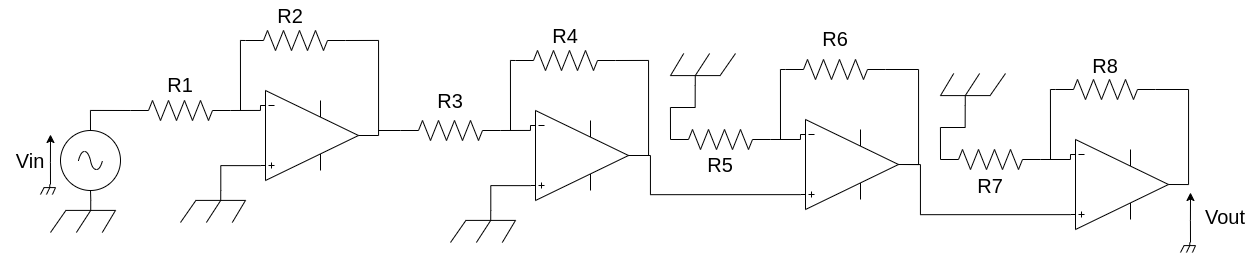
\includegraphics[width=\textwidth]{chaine-AOP.drawio.png}

La dernière étape consiste à \textit{dimensionner} les résistances afin d'obtenir des gains adéquats.
Nous pouvons par exemple choisir les gains suivants~:
\begin{center}
\begin{tabular}{|l|cccc|}\hline
Étage & 1 & 2 & 3 & 4 \\
Gain & 50 & 50 & 20 & 10 \\ \hline
\end{tabular}
\end{center}

Les deux premiers étages sont des inverseurs~: $\left|\frac{-R_2}{R_1}\right| = 50$ et $\left|\frac{-R_4}{R_3}\right| = 50$.
Prenons des valeurs de résistance réalistes~:
\begin{center}
\begin{tabular}{|cccc|}\hline
$R_1$ & $R_2$ & $R_3$ & $R_4$ \\
$1 k\Omega$ & $50 k\Omega$ & $1 k\Omega$ & $50 k\Omega$ \\ \hline
\end{tabular}
\end{center}

Les deux derniers étages sont des non-inverseurs dont le gain est $1 + \frac{R_6}{R_5} = 20$ et $1 + \frac{R_8}{R_7} = 10$.
Nous pouvons alors choisir~:
\begin{center}
\begin{tabular}{|cccc|}\hline
$R_5$ & $R_6$ & $R_7$ & $R_8$ \\
$1k k\Omega$ & $19 k\Omega$ & $1 k\Omega$ & $90 k\Omega$ \\ \hline
\end{tabular}
\end{center}


\Question{0}
{
On a un signal de valeur maximale $1\ mV$ et composé de sinusoïdes dont les fréquences vont jusque $100\ kHz$. La source de laquelle sort ce signal a une impédance de sortie de $1\ k\Omega$.\\
On souhaite avoir en sortie du montage un signal fidèle à celui d'entrée mais d'une amplitude ajustable allant de  $0\ V$ à $1\ V$.\\

Pour réaliser le montage amplificateur on dispose uniquement:
\begin{itemize}
    \item d'amplificateurs opérationnels de produit gain bande passante $GPB=1MHz$;
    \item de résistances de $1\ k\Omega$, de $9\ k\Omega$ et de $10\ k\Omega$;
    \item de potentiomètres de $10\ k\Omega$;
    \item et d'un protoboard alimenté en $+12/-12\ V$ et de quelques fils pour pouvoir réaliser le montage amplicateur.
\end{itemize}

Dimensionnez et dessinez ce montage amplificateur en utilisant le moins de composants possible.

\textit{-- Question d'examen d'août 2019}
}
{
  Le gain total du montage doit donc être de:
$$G_{tot}\frac{\hat{V}_{out}}{\hat{V}_{in}}=\frac{1\ V}{1\ mV}=1000$$

Avec un AOP, j'ai un gain maximum de:
$$G_{1AOP}=\frac{GBP}{BP}=\frac{1MHz}{100kHz}=10$$
Il va donc falloir au minimum 3 étages à AOP car
$$|G_{1AOP}=10| < |G_{2AOP}=10^2=100| < |G_{tot}=1000| = |G_{3AOP}|=10^3$$

Il faut donc 3 étages de gain $10$, cela est possible:
\begin{itemize}
    \item aussi bien avec des inverseurs en prenant une résistance $R_2=10\ k\Omega$ et une résistance $R_1=1\ k\Omega$, tel que le gain soit: $G_I=\frac{-R_2}{R_1}=-10$,
    \item qu'avec des non inverseurs en prenant une résistance $R_2=9\ k\Omega$ et une résistance $R_1=1\ k\Omega$, tel que le gain soit: $G_{NI}=1+\frac{R_2}{R_1}=10$.
\end{itemize}

Vu que l'impédance de sortie de la source vaut $1\ k\Omega$ (comme $R_1$), le premier étage doit être un non inverseur qui a une impédance d'entrée infinie (ou utilise un suiveur mais ça ajouterait un AOP au circuit).\\
En effet, l'utilisation d'un étage inverseur de $R_1=1\ k\Omega$ créerait un diviseur de tension qui diminuerait l'amplitude de la tension d'entrée de 1/11ème ($\frac{10k}{k10k+1k}=\frac{10}{11}$).\\
Le gain de ce premier étage est donc:
$$G_{1,NI}=1+\frac{R_2}{R_1}=1+\frac{9k}{1k}=10$$

Etant donné que l'amplitude du signal doit pouvoir être annulé, il faut au moins un étage inverseur avec potentiomètre dans le montage. Son gain est:
$$G_{I,2}=\frac{-P}{R_3}=\frac{-[0\rightarrow 10k]}{1k}=[0\rightarrow -10]$$

Le dernier étage doit également être un inverseur étant donné que le signal de sortie doit être fidèle au signal d'entrée (pas d'inversion). Son gain est donc:
$$G_{I,3}=\frac{-R_5}{R_4}=\frac{-10k}{1k}=-10$$


\begin{center}
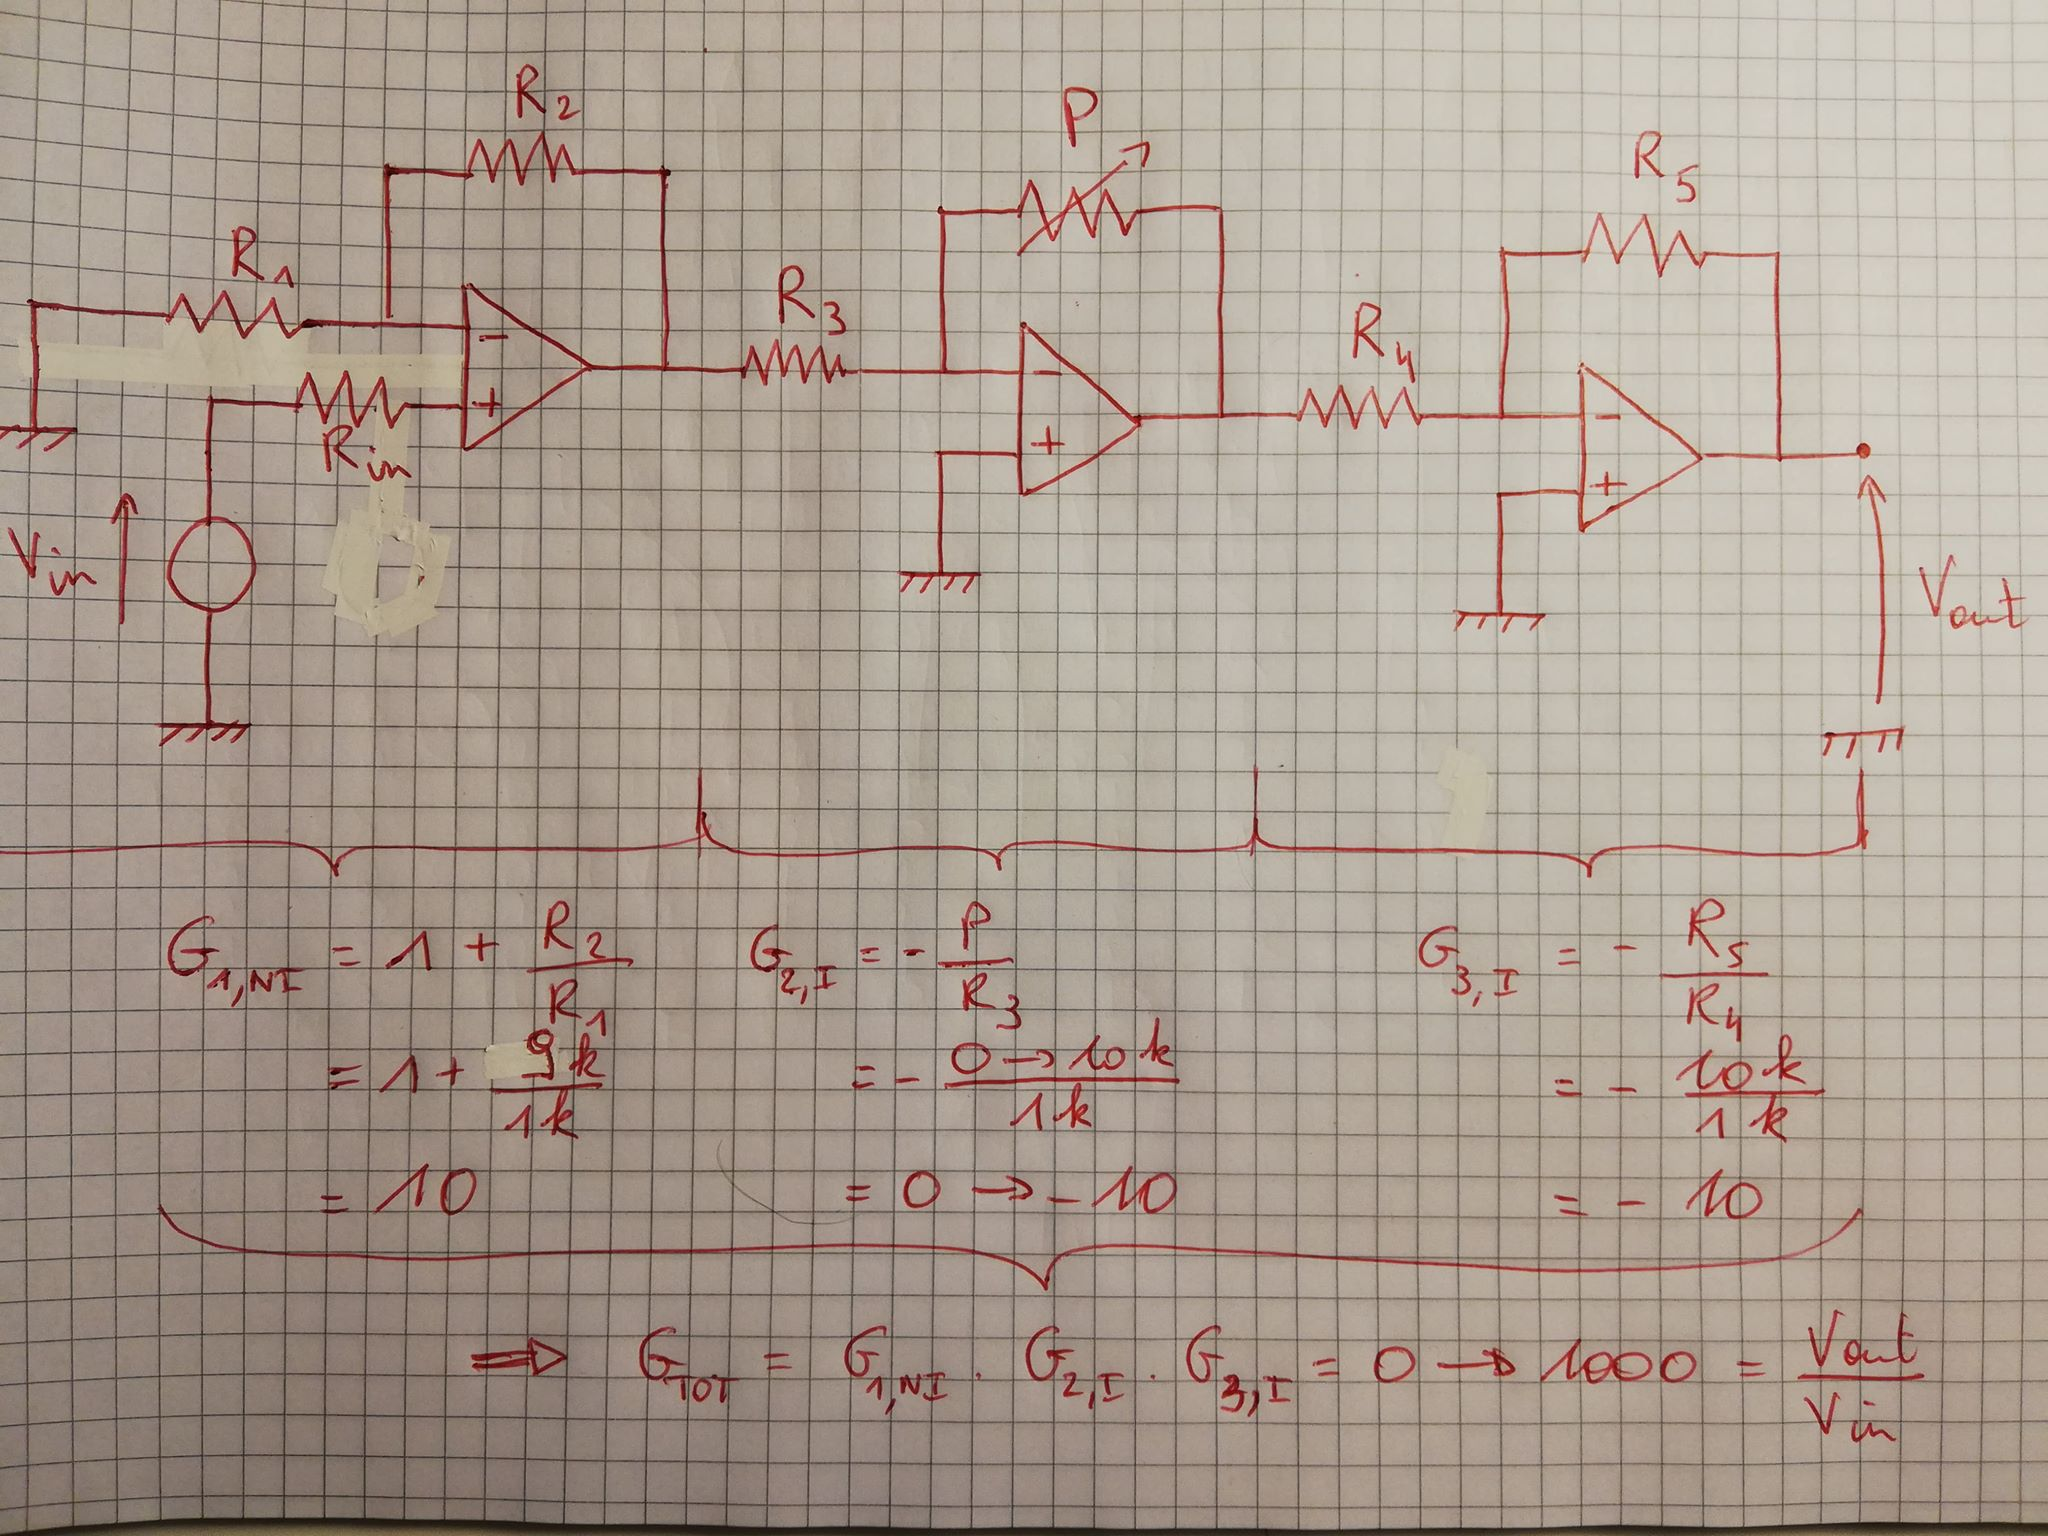
\includegraphics[width=.9\textwidth]{AOP2.jpg}
\end{center}

}



\endinput
